\section{Diseño del proyecto, primera iteración}

\subsection{Análisis del problema y de los datos}\label{sec:obtencion}

Considerando que los datos contenidos en los archivos \acrshort{bil} que hemos recibido desde el laboratorio contienen 168 columnas con información de las diferentes longitudes de onda\ \cite{WhatIsHy18:online} y además el nivel de contaminación \gls{don} de cada grano, podemos generar un \gls{dataset} con los datos de cada grano, haciendo la media de cada longitud de onda por cada píxel del mismo grano. Una vez hemos extraído la información de todos los archivos \acrshort{bil} y la hemos guardado en un archivo \acrshort{csv}, podemos entrenar los modelos.

Cabe recalcar que para los modelos de regresión nos hemos guardado el valor de contaminación \gls{don} explícitamente, para los de clasificación si el valor \gls{don} supera los límites de contaminación y hemos preparado un \gls{dataset} aparte con algunos archivos \gls{bil} que contienen granos que no han sido analizados químicamente para el entrenamiento semi-supervisado.

En esta primera iteración nos hemos centrado en intentar encontrar un buen modelo de clasificación y mejorar sus resultados lo máximo posible.

\subsection{Preprocesado de datos}\label{sec:preprocesado}

Ahora que tenemos los datos en un solo archivo \acrshort{csv}, el siguiente paso es preparar los datos. Para ello, hemos realizado el siguiente proceso: 

\begin{enumerate}
    \item Eliminación de columnas
    \item Codificación
    \item Valores atípicos (\textit{outliers})
    \item Balanceo de datos
    \item Separación en datos de entreno y de prueba (\textit{train-test-split})
    \item Preprocesado común, (\textit{pipeline})
    \begin{enumerate}
        \item Separación de datos aplicando la primera derivada 
        \item Aumento de dimensionalidad (\textit{Polynomial Features})
        \item Estandarización  (\textit{Standard Scaler})
        \item Reducción de dimensionalidad (\textit{Principal Component Analysis})
    \end{enumerate}
    
\end{enumerate}


\subsubsection{Eliminación de columnas, codificación y valores atípicos}

Existen datos que nos interesan como medida de seguridad, pero no nos interesa que un modelo entrene con ellos, ya que podría inferir patrones irreales o incluso memorizárselos y hacer \gls{overfitting}. En nuestro caso, un ejemplo sería una columna que indicase el número identificador del grano o el archivo del cual se han extraído los datos.

La codificación consiste en transformar columnas con datos categóricos en columnas de datos numéricos, pues los modelos de \acrshort{ml} funcionan mejor con valores numéricos. En nuestro caso, la única columna con valores no numéricos era la columna de la contaminación, que podía tomar los valores \textit{\{B, C\}}, así que lo codificamos manualmente como se muestra a continuación:

{\centering
    \textit{B \longrightarrow{} 0}, \textit{C \longrightarrow{} 1}\par
}

Los valores atípicos u \textit{outliers} son aquellos valores inusuales en los datos que pueden distorsionar nuestros análisis estadísticos. Sin embargo, se debe tener en cuenta que puede haber mucha variación en la naturaleza de nuestro problema. Por ello, se deben diferenciar los \textit{outliers} que se pueden incluir en los datos y los que no. En nuestro caso, los hemos incluido todos, pues al tener cada grano 168 columnas de datos, la mayoría tenía alguna columna que no entraba dentro de lo ``normal'', como por ejemplo en la \textit{figura\ \ref{fig:outliers}}. Por lo que después de probar a quitar todos los granos que alguna de sus columnas fuera un \textit{outlier} (con el \textit{código\ \ref{code:zscore}}), nos quedamos sin datos.

\begin{figure}[!htb]
    \centering
    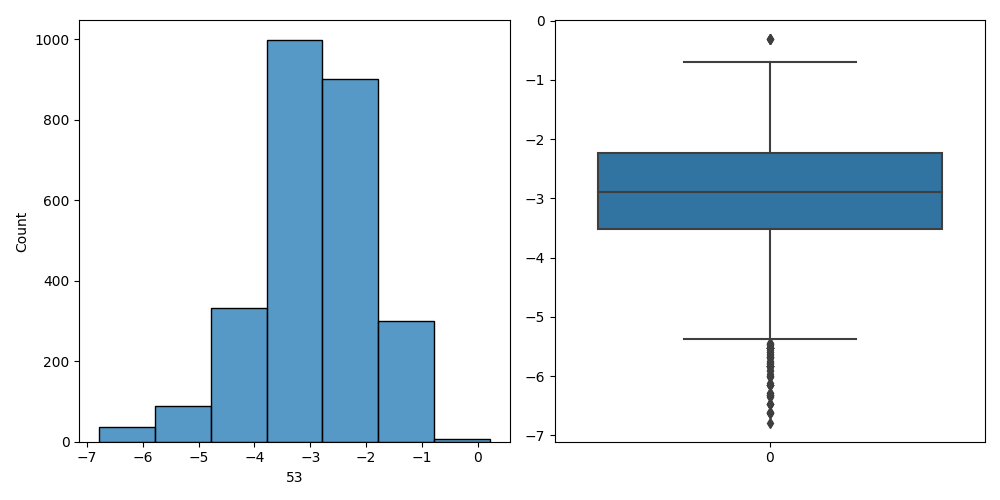
\includegraphics[width=0.7\linewidth]{media/images/col-53-outliers.png}
    \caption{Representación de los \textit{outliers} de la columna 53 en un gráfico de velas, fuente propia, \textit{código\ \ref{code:plot-outliers}}}\ \label{fig:outliers}
\end{figure}


\subsubsection{Balanceo de datos}

Podemos ver en la \textit{figura\ \ref{fig:unbalance}} que los datos no están balanceados, es decir, que la columna que nos interesa `Contaminación' no tiene un número de datos similares en cada clase. En nuestro caso, como en general es más complicado encontrarse un grano contaminado, tenemos más granos sanos.

Al tener las clases desbalanceadas tenemos varias opciones:
\begin{enumerate}
    \item Usar métodos de evaluación que tengan en cuenta el desbalance de las clases.
    \item Balancear el \gls{dataset} utilizando tanto \textit{undersampling} como \textit{oversampling} (explicados en el \textit{apartado\ \ref{sec:i2-balance}}).
\end{enumerate}

Para esta primera iteración, nos es más sencillo utilizar métricas que tengan en cuenta el número de instancias de cada clase a la hora de evaluar los resultados, es decir, que tengan en cuenta el desbalance del \gls{dataset}.

\begin{figure}[!ht]
    \centering
    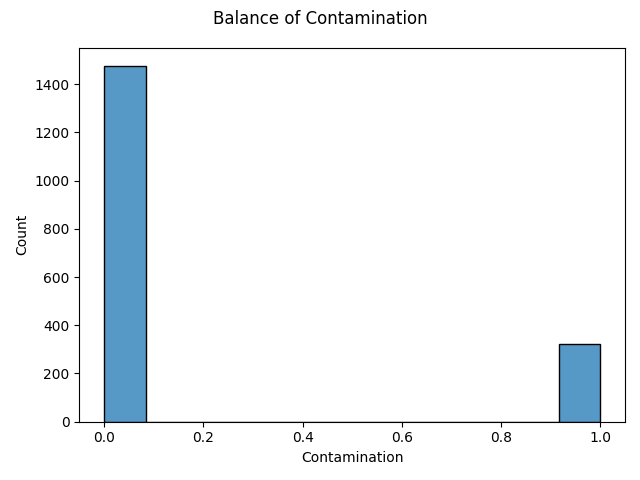
\includegraphics[width=0.7\linewidth]{media/images/unabalance.png}
    \caption{Balanceo de la clase objetivo del \gls{dataset}, fuente propia}\ \label{fig:unbalance}
\end{figure}


\subsubsection{Separación de datos de entreno y de prueba}

En todo el proyecto hemos estado utilizando la librería \href{https://scikit-learn.org/stable/}{sklearn}, esta tiene un submódulo con una función \href{https://scikit-learn.org/stable/modules/generated/sklearn.model_selection.train_test_split.html}{sklearn.model\_selection.train\_test\_split} para separar el \gls{dataset} en entreno y prueba. De todas las opciones, cabe recalcar una que hemos habilitado, pues como en el \gls{dataset} original las etiquetas no están balanceadas y hay muchos más granos sanos que contaminados, es importante que los granos contaminados estén igualmente representados tanto en el conjunto de prueba como en el de entreno. Esto se consigue con la opción \textit{stratify}.


\subsubsection{Preprocesado común}

Después de balancear los datos, debemos transformarlos para que tengan algunas propiedades que suelen ser preferibles a la hora de entrenar ciertos modelos. Es decir, hay modelos que les vendrá mejor tener los datos estandarizados, por ejemplo, y otros que no hará falta o será contraproducente, al final será la prueba y error lo que nos diga qué pasos son preferibles.

Antes de probar diferentes formas de preprocesar los datos, hemos preparado un entorno para entrenar una batería de modelos distintos para ver su efectividad.

Un primer paso, recomendado desde el laboratorio, ya que era lo que utilizaban ellos en su modelo estadístico, es aplicar la primera derivada. El aplicar la derivada permite mínimamente separar los granos contaminados de los que no. Para probarlo, podemos comparar los resultados de entrenar con o sin derivar en la \textit{tabla\ \ref{tab:nopreprocessing-derivative-results}} y, efectivamente, obtenemos resultados algo mejores.

\begin{table}[!ht]
    \centering
    \resizebox{\textwidth}{!}{\begin{tabular}{|c|ccccccc|ccccccc|}
        \hline
        & \multicolumn{7}{|c|}{Derivative} & \multicolumn{7}{c|}{No preprocessing} \\ \hline
        Model Name & Train score & Test score & f1score & f0.5score & f2score & ROC/AUC score & Balanced accuracy & Train score & Test score & f1score & f0.5score & f2score & ROC/AUC score & Balanced accuracy \\ \hline
        XGBoost & 82 & 82 & 0 & 0 & 0 & 50 & 50 & 82 & 82 & 0 & 0 & 0 & 50 & 50 \\
        Stochastic Gradient Descent & 18 & 18 & 30.508 & 21.531 & 52.326 & 50 & 50 & 18 & 18 & 30.508 & 21.531 & 52.326 & 50 & 50 \\
        Random Forest & 99.926 & 87.778 & 49.541 & 69.948 & 38.352 & 66.531 & 66.531 & 99.556 & 84.889 & 52.778 & 57.057 & 49.096 & 70.069 & 70.069 \\
        Quadratic Discriminant Analysis & 100 & 82 & 0 & 0 & 0 & 50 & 50 & 100 & 82 & 0 & 0 & 0 & 50 & 50 \\
        Multi-Layer Perceptron & 83.259 & 80.667 & 8.421 & 14.599 & 5.917 & 51.114 & 51.114 & 82 & 82 & 0 & 0 & 0 & 50 & 50 \\
        Linear Discriminant Analysis & 85.333 & 78.222 & 20.968 & 25.692 & 17.711 & 53.96 & 53.96 & 84.889 & 78 & 22.047 & 26.415 & 18.919 & 54.306 & 54.306 \\
        LightGBM & 81.852 & 72 & 47.934 & 40 & 59.794 & 71.846 & 71.846 & 75.778 & 64 & 37.692 & 30.74 & 48.708 & 62.632 & 62.632 \\
        K-Neighbors & 100 & 86.889 & 56.296 & 63.973 & 50.265 & 71.289 & 71.289 & 100 & 91.778 & 74.83 & 79.71 & 70.513 & 82.46 & 82.46 \\
        Hist Gradient Boosting & 78.444 & 70.444 & 44.813 & 37.448 & 55.785 & 68.97 & 68.97 & 72.815 & 63.556 & 33.871 & 28.037 & 42.77 & 58.988 & 58.988 \\
        Extra Trees & 99.63 & 90.444 & 69.504 & 76.324 & 63.802 & 78.756 & 78.756 & 94.667 & 81.111 & 56.853 & 51.376 & 63.636 & 76.438 & 76.438 \\
        Decision Tree & 56.963 & 58.889 & 41.27 & 31.957 & 58.244 & 67.224 & 67.224 & 82 & 82 & 0 & 0 & 0 & 50 & 50 \\ \hline
        & & & & & & 61.79 & 61.79 & & & & & & 59.53572727 & 59.53572727 \\ \hline
        \end{tabular}}
    \caption{Comparación de los resultados de entrenar utilizando la derivada y sin preprocesar. Fuente propia.}\ \label{tab:nopreprocessing-derivative-results}
\end{table}


El siguiente paso que podemos probar es aplicar la transformada, como los resultados habiendo derivado los datos son mejores, transformaremos los datos después de derivarlos. Podríamos probar todas las permutaciones de los diferentes pasos de preprocesado, sin embargo, en esta primera iteración tan solo nos interesa encontrar un resultado decente. Podríamos hacerlo en una segunda o tercera iteración si lo vemos necesario. La transformada consiste en transformar cada columna para que tengan una forma gaussiana\ \cite{sklearnp39:online}. Como estamos utilizando \textit{sklearn}, tenemos una clase que nos aplica la transformada \href{https://scikit-learn.org/stable/modules/generated/sklearn.preprocessing.PowerTransformer.html}{sklearn.preprocessing.PowerTransformer}, por defecto esta clase además te aplica una estandardización de los datos, pero la hemos deshabilitado para aplicarla en otro paso. Podemos ver los resultados de entrenar utilizando la derivada y transformada en la \textit{tabla\ \ref{tab:derivative-transformed-results}}, podemos ver que los resultados son peores, así que continuaremos las pruebas con la derivada.

\begin{table}[!ht]
    \centering
    \resizebox{\textwidth}{!}{\begin{tabular}{|c|ccccccc|ccccccc|}
        \hline
            & \multicolumn{7}{|c|}{Transformer and derivative} & \multicolumn{7}{c|}{Derivative} \\ \hline
            Model Name & Train score & Test score & f1score & f0.5score & f2score & ROC/AUC score & Balanced accuracy & Train score & Test score & f1score & f0.5score & f2score & ROC/AUC score & Balanced accuracy \\ \hline
            XGBoost & 82 & 82 & 0 & 0 & 0 & 50 & 50 & 82 & 82 & 0 & 0 & 0 & 50 & 50 \\
            Stochastic Gradient Descent & 18 & 18 & 30.508 & 21.531 & 52.326 & 50 & 50 & 18 & 18 & 30.508 & 21.531 & 52.326 & 50 & 50 \\
            Random Forest & 99.926 & 87.778 & 49.541 & 69.948 & 38.352 & 66.531 & 66.531 & 99.926 & 87.778 & 49.541 & 69.948 & 38.352 & 66.531 & 66.531 \\
            Quadratic Discriminant Analysis & 100 & 83.333 & 19.355 & 34.884 & 13.393 & 55.149 & 55.149 & 100 & 82 & 0 & 0 & 0 & 50 & 50 \\
            Multi-Layer Perceptron & 82 & 82 & 0 & 0 & 0 & 50 & 50 & 83.259 & 80.667 & 8.421 & 14.599 & 5.917 & 51.114 & 51.114 \\
            Linear Discriminant Analysis & 85.185 & 76.667 & 18.605 & 21.978 & 16.129 & 52.529 & 52.529 & 85.333 & 78.222 & 20.968 & 25.692 & 17.711 & 53.96 & 53.96 \\
            LightGBM & 81.852 & 72 & 47.934 & 40 & 59.794 & 71.846 & 71.846 & 81.852 & 72 & 47.934 & 40 & 59.794 & 71.846 & 71.846 \\
            K-Neighbors & 100 & 80.222 & 25.21 & 32.189 & 20.718 & 56.143 & 56.143 & 100 & 86.889 & 56.296 & 63.973 & 50.265 & 71.289 & 71.289 \\
            Hist Gradient Boosting & 78.444 & 70.444 & 44.813 & 37.448 & 55.785 & 68.97 & 68.97 & 78.444 & 70.444 & 44.813 & 37.448 & 55.785 & 68.97 & 68.97 \\
            Extra Trees & 99.63 & 90 & 68.966 & 74.184 & 64.433 & 78.967 & 78.967 & 99.63 & 90.444 & 69.504 & 76.324 & 63.802 & 78.756 & 78.756 \\
            Decision Tree & 56.963 & 58.889 & 41.27 & 31.957 & 58.244 & 67.224 & 67.224 & 56.963 & 58.889 & 41.27 & 31.957 & 58.244 & 67.224 & 67.224 \\ \hline
            & & & & & & 60.669 & 60.669 & & & & & & 61.79 & 61.79 \\ \hline
        \end{tabular}}
    \caption{Comparación de los resultados de entrenar transformando y derivando los datos; frente a solo derivando. Fuente propia.}\ \label{tab:derivative-transformed-results}
\end{table}

A continuación, probaremos la estandarización de los datos como hemos comentado anteriormente. Utilizaremos la clase \href{https://scikit-learn.org/stable/modules/generated/sklearn.preprocessing.StandardScaler.html}{sklearn.preprocessing.StandardScaler}.
La estandardización consiste en el centrado y escalado de los datos. Para ello, columna por columna, restamos la media de los valores (centramos en torno al 0) y 
los dividimos por la varianza (para que la desviación tienda a 1). Tener los datos estandarizados es suele ser un requisito para obtener buenos resultados al entrenar algunos modelos.\ \cite{sklearnp24:online}
Como consecuencia, en la \textit{tabla\ \ref{tab:derivative-standarization-results}} podemos ver que obtenemos mejores resultados.


\begin{table}[!ht]
    \resizebox{\textwidth}{!}{\begin{tabular}{|c|ccccccc|ccccccc|}
        \hline
        & \multicolumn{7}{c|}{Derivative + Scaler} & \multicolumn{7}{c|}{Derivative} \\ \hline
        Model Name & Train score & Test score & f1score & f0.5score & f2score & ROC/AUC score & Balanced accuracy & Train score & Test score & f1score & f0.5score & f2score & ROC/AUC score & Balanced accuracy \\ \hline
        XGBoost & 82 & 82 & 0 & 0 & 0 & 50 & 50 & 82 & 82 & 0 & 0 & 0 & 50 & 50 \\
        Stochastic Gradient Descent & 64.815 & 56.444 & 24.615 & 20.075 & 31.809 & 49.834 & 49.834 & 18 & 18 & 30.508 & 21.531 & 52.326 & 50 & 50 \\
        Random Forest & 99.926 & 87.778 & 49.541 & 69.948 & 38.352 & 66.531 & 66.531 & 99.926 & 87.778 & 49.541 & 69.948 & 38.352 & 66.531 & 66.531 \\
        Quadratic Discriminant Analysis & 96.148 & 83.111 & 54.217 & 53.444 & 55.012 & 72.358 & 72.358 & 100 & 82 & 0 & 0 & 0 & 50 & 50 \\
        Multi-Layer Perceptron & 90.815 & 84 & 32.075 & 46.961 & 24.355 & 59.41 & 59.41 & 83.259 & 80.667 & 8.421 & 14.599 & 5.917 & 51.114 & 51.114 \\
        Linear Discriminant Analysis & 85.333 & 78.222 & 20.968 & 25.692 & 17.711 & 53.96 & 53.96 & 85.333 & 78.222 & 20.968 & 25.692 & 17.711 & 53.96 & 53.96 \\
        LightGBM & 82.222 & 72.222 & 48.133 & 40.222 & 59.917 & 71.981 & 71.981 & 81.852 & 72 & 47.934 & 40 & 59.794 & 71.846 & 71.846 \\
        K-Neighbors & 100 & 86.889 & 55.639 & 64.014 & 49.202 & 70.807 & 70.807 & 100 & 86.889 & 56.296 & 63.973 & 50.265 & 71.289 & 71.289 \\
        Hist Gradient Boosting & 78.444 & 70.444 & 44.813 & 37.448 & 55.785 & 68.97 & 68.97 & 78.444 & 70.444 & 44.813 & 37.448 & 55.785 & 68.97 & 68.97 \\
        Extra Trees & 99.63 & 90.444 & 69.504 & 76.324 & 63.802 & 78.756 & 78.756 & 99.63 & 90.444 & 69.504 & 76.324 & 63.802 & 78.756 & 78.756 \\
        Decision Tree & 56.963 & 58.889 & 41.27 & 31.957 & 58.244 & 67.224 & 67.224 & 56.963 & 58.889 & 41.27 & 31.957 & 58.244 & 67.224 & 67.224 \\ \hline
        & & & & & & 64.53009091 & 64.53009091 & & & & & & 61.79 & 61.79 \\ \hline
        \end{tabular}}
    \caption{Comparación de los resultados de entrenar derivando y estandarizando los datos; frente a solo derivando. Fuente propia.}\ \label{tab:derivative-standarization-results}
\end{table}


Además, podemos probar dos últimos pasos que suelen ir juntos. El primero, \href{https://scikit-learn.org/stable/modules/generated/sklearn.preprocessing.PolynomialFeatures.html}{sklearn.preprocessing.PolynomialFeatures}, 
nos permite generar nuevas columnas de datos que consisten en combinar las demás columnas, multiplicándolas entre sí y elevando a un grado específico (segundo grado en nuestro caso). 
De esta forma, teníamos un \gls{dataset} de 168 columnas y obtenemos uno de 14365 columnas. Por ello, debemos aplicar el segundo y último paso para reducir la dimensionalidad
de los datos. Este paso es \href{https://scikit-learn.org/stable/modules/generated/sklearn.decomposition.PCA.html}{sklearn.decomposition.PCA} o \textit{Principal Component Analysis},
reduce la dimensionalidad proyectando los datos a una espacio de menor dimensionalidad. Explicar este proceso más detenidamente se va de nuestro objetivo, pero
aquí podemos leer algo más al respecto sobre \textit{PCA} en \ \cite{Principa62:online}.
Aun añadiendo complejidad de esta forma, podemos ver en la \textit{tabla \ref{tab:derivative-standarization-dimensionality-results}} que los resultados son mejores si
nos quedamos en el paso anterior.

\begin{table}[!ht]
    \resizebox{\textwidth}{!}{\begin{tabular}{|c|ccccccc|ccccccc|}
        \hline
            & \multicolumn{7}{c}{Derivative + Scaler + Polynomial Features + PCA} & \multicolumn{7}{c}{Derivative + Scaler} \\ \hline
            Model Name & Train score & Test score & f1score & f0.5score & f2score & ROC/AUC score & Balanced accuracy & Train score & Test score & f1score & f0.5score & f2score & ROC/AUC score & Balanced accuracy \\ \hline
            XGBoost & 82 & 82 & 0 & 0 & 0 & 50 & 50 & 82 & 82 & 0 & 0 & 0 & 50 & 50 \\
            Stochastic Gradient Descent & 53.333 & 50.444 & 28.754 & 22.299 & 40.468 & 52.439 & 52.439 & 64.815 & 56.444 & 24.615 & 20.075 & 31.809 & 49.834 & 49.834 \\
            Random Forest & 99.926 & 85.778 & 38.462 & 57.803 & 28.818 & 61.939 & 61.939 & 99.926 & 87.778 & 49.541 & 69.948 & 38.352 & 66.531 & 66.531 \\
            Quadratic Discriminant Analysis & 80.889 & 80 & 40 & 42.017 & 38.168 & 63.234 & 63.234 & 96.148 & 83.111 & 54.217 & 53.444 & 55.012 & 72.358 & 72.358 \\
            Multi-Layer Perceptron & 87.778 & 81.778 & 19.608 & 30.303 & 14.493 & 54.682 & 54.682 & 90.815 & 84 & 32.075 & 46.961 & 24.355 & 59.41 & 59.41 \\
            Linear Discriminant Analysis & 82.741 & 81.111 & 6.593 & 12.397 & 4.491 & 50.903 & 50.903 & 85.333 & 78.222 & 20.968 & 25.692 & 17.711 & 53.96 & 53.96 \\
            LightGBM & 77.037 & 68.444 & 38.261 & 32.496 & 46.512 & 62.933 & 62.933 & 82.222 & 72.222 & 48.133 & 40.222 & 59.917 & 71.981 & 71.981 \\
            K-Neighbors & 100 & 83.778 & 42.52 & 50.943 & 36.486 & 64.092 & 64.092 & 100 & 86.889 & 55.639 & 64.014 & 49.202 & 70.807 & 70.807 \\
            Hist Gradient Boosting & 75.63 & 66 & 37.037 & 30.864 & 46.296 & 61.924 & 61.924 & 78.444 & 70.444 & 44.813 & 37.448 & 55.785 & 68.97 & 68.97 \\
            Extra Trees & 96.222 & 82.222 & 51.22 & 50.847 & 51.597 & 70.37 & 70.37 & 99.63 & 90.444 & 69.504 & 76.324 & 63.802 & 78.756 & 78.756 \\
            Decision Tree & 71.852 & 68.889 & 27.835 & 25.328 & 30.892 & 55.014 & 55.014 & 56.963 & 58.889 & 41.27 & 31.957 & 58.244 & 67.224 & 67.224 \\ \hline
            & & & & & & 58.86636364 & 58.86636364 & & & & & & 64.53009091 & 64.53009091 \\ \hline
        \end{tabular}} 
    \caption{Comparación de los resultados de entrenar derivando, estandarizando y ajustando la dimensionalidad de los datos; frente a solo derivando y estandarizando. Fuente propia.}\ \label{tab:derivative-standarization-dimensionality-results}
\end{table}



\href{https://scikit-learn.org/stable/modules/generated/sklearn.pipeline.Pipeline.html}{Pipeline}


\subsection{Entrenamiento de modelos, selección e \textit{hypertuning}}\ \label{sec:entrenamiento}

Ahora que tenemos los datos preparados, podemos entrenar modelos. Aunque hay muchos tipos de modelos preparados en la librería, cada uno funciona de una forma. Podríamos investigar cuál funciona mejor con nuestros datos, sin embargo, como el \gls{dataset} que tenemos no es muy grande, podemos entrenar todos sin perder mucho tiempo y mirar cuál tiene mejores resultados. Estos resultados del primer entrenamiento los podemos ver en la \textit{tabla\ \ref{tab:first-model-training}}

\begin{table}[!ht]
    \centering
    \resizebox{\textwidth}{!}{\begin{tabular}{|ll|llllllll|l|}
        \hline~& Model Name & Train score & Test score & Recall & Precision & f1score & f0.5score & f2score & ROC/AUC score & Balanced accuracy \\ \hline
            mlp & Multi-Layer Perceptron & 91.902 & 90.707 & 86.15 & 94.817 & 90.276 & 92.947 & 87.754 & 90.714 & 90.714 \\ \hline
            xgb & XGBoost & 92.226 & 88.904 & 84.211 & 92.966 & 88.372 & 91.072 & 85.827 & 88.911 & 88.911 \\ \hline
            rf & Random Forest & 94.678 & 88.766 & 83.38 & 93.478 & 88.141 & 91.267 & 85.221 & 88.773 & 88.773 \\ \hline
            lgbm & LightGBM & 91.856 & 88.488 & 84.488 & 91.867 & 88.023 & 90.29 & 85.867 & 88.494 & 88.494 \\ \hline
            qda & Quadratic Discriminant Analysis & 87.043 & 88.488 & 77.839 & 98.944 & 87.132 & 93.854 & 81.308 & 88.503 & 88.503 \\ \hline
            et & Extra Trees model & 85.886 & 85.437 & 78.116 & 91.558 & 84.305 & 88.512 & 80.479 & 85.447 & 85.447 \\ \hline
            knn & K-Neighbors & 100.0 & 83.218 & 70.36 & 94.776 & 80.763 & 88.625 & 74.182 & 83.236 & 83.236 \\ \hline
            hgb & Hist Gradient Boosting & 81.259 & 82.802 & 76.177 & 87.859 & 81.602 & 85.245 & 78.258 & 82.811 & 82.811 \\ \hline
            lda & Linear Discriminant Analysis & 80.102 & 82.802 & 73.961 & 89.899 & 81.155 & 86.185 & 76.68 & 82.814 & 82.814 \\ \hline
            sgd & Stochastic Gradient Descent & 76.955 & 80.999 & 73.961 & 86.129 & 79.583 & 83.385 & 76.112 & 81.008 & 81.008 \\ \hline
            dt & Decision Tree & 72.975 & 76.144 & 62.05 & 86.486 & 72.258 & 80.172 & 65.766 & 76.164 & 76.164 \\ \hline
        \end{tabular}}
    \caption{Resultados del primer entrenamiento de modelos. Fuente propia.}\ \label{tab:first-model-training}
\end{table}

Una vez hemos entrenado estos modelos vemos que hay muchos que hacen \textit{overfitting}, para verlo más claramente podemos ver sus curvas de aprendizaje en la \textit{figura\ \ref{fig:learning-curves}}. La que más claramente se ve es en la \textit{figura\ \ref{sfig:lc-knn}}, nos hemos de fijar en la diferencia de resultados en el \gls{dataset} sobre el que se ha entrenado y el de prueba. Para evitar el \gls{overfitting} vamos a seleccionar los mejores modelos y a hacer \textit{hyperparameter tuning}. 

\begin{figure}[!ht]
    \centering
    \begin{subfigure}[b]{0.3\textwidth}
        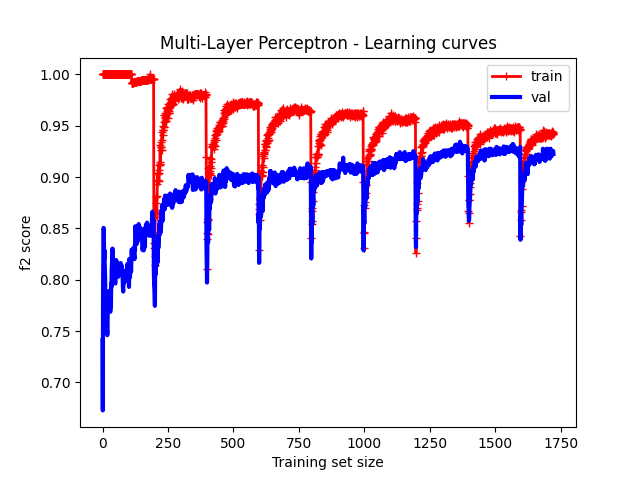
\includegraphics[width=\linewidth]{media/images/learning-curves/mlp.png}
        \caption{Curva de aprendizaje del Multilayer Perceptron}\ \label{sfig:lc-mlp}
    \end{subfigure}
    \begin{subfigure}[b]{0.3\textwidth}
        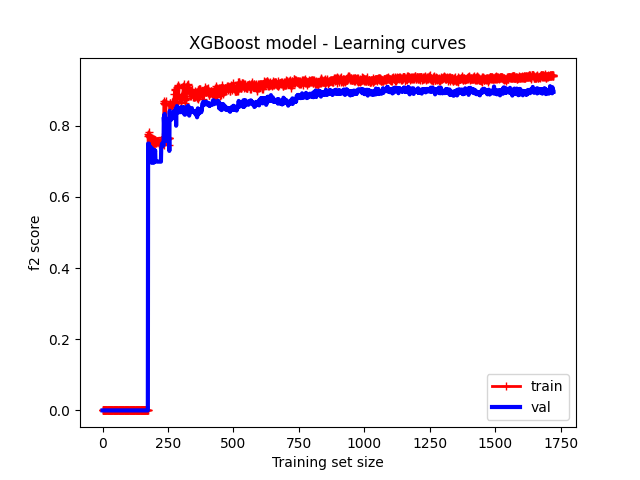
\includegraphics[width=\linewidth]{media/images/learning-curves/xgb.png}
        \caption{Curva de aprendizaje del XGBoost}\ \label{sfig:lc-xgb}
    \end{subfigure}
    \begin{subfigure}[b]{0.3\textwidth}
        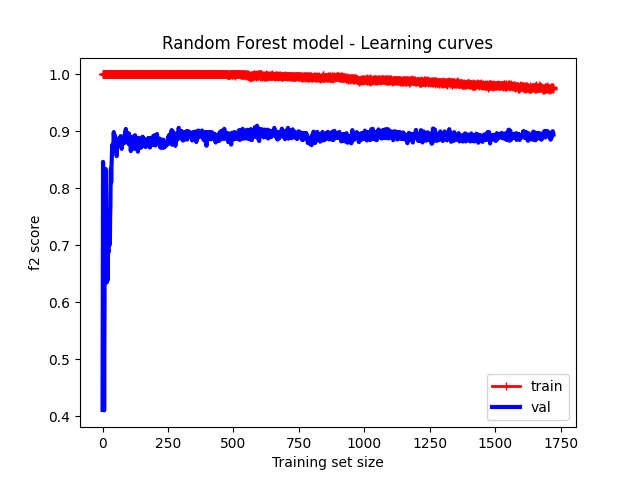
\includegraphics[width=\linewidth]{media/images/learning-curves/rf.png}
        \caption{Curva de aprendizaje del Random Forest}\ \label{sfig:lc-rf}
    \end{subfigure}
    \begin{subfigure}[b]{0.3\textwidth}
        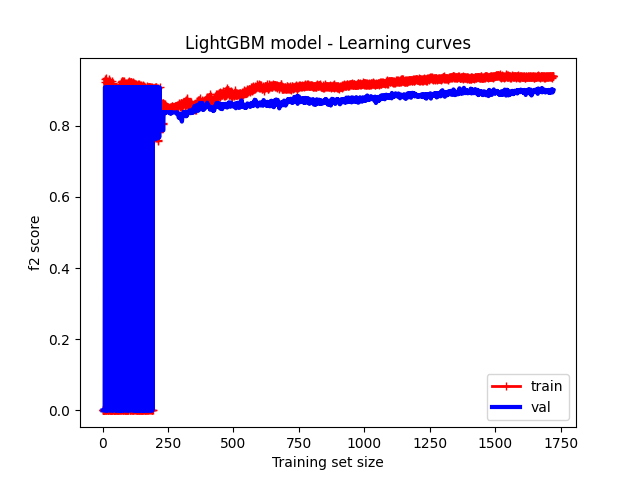
\includegraphics[width=\linewidth]{media/images/learning-curves/lgbm.png}
        \caption{Curva de aprendizaje del LightGBM}\ \label{sfig:lc-lgbm}
    \end{subfigure}
    \begin{subfigure}[b]{0.3\textwidth}
        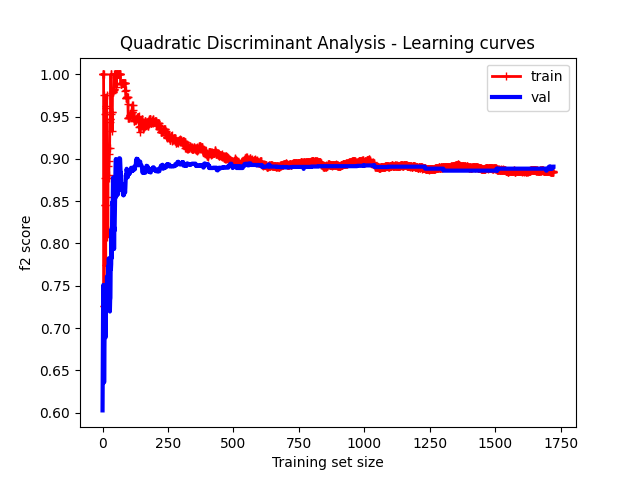
\includegraphics[width=\linewidth]{media/images/learning-curves/qda.png}
        \caption{Curva de aprendizaje del Quadratic Discriminant Analysis}\ \label{sfig:lc-qda}
    \end{subfigure}
    \begin{subfigure}[b]{0.3\textwidth}
        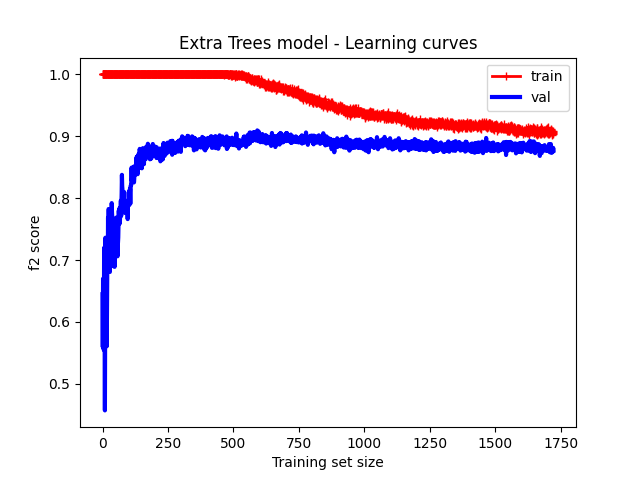
\includegraphics[width=\linewidth]{media/images/learning-curves/et.png}
        \caption{Curva de aprendizaje del Extra Trees}\ \label{sfig:lc-et}
    \end{subfigure}
    \begin{subfigure}[b]{0.3\textwidth}
        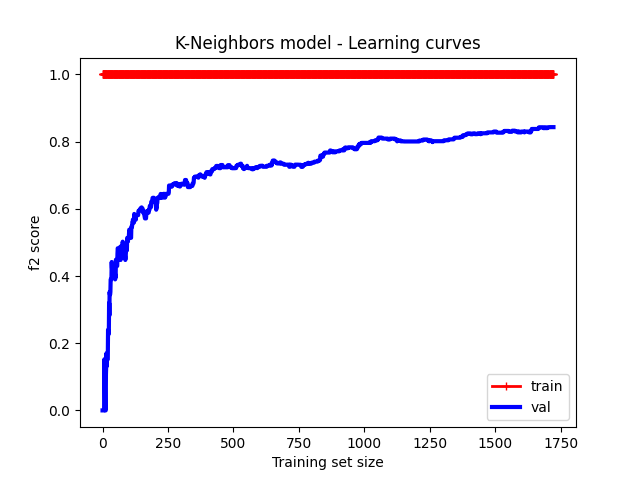
\includegraphics[width=\linewidth]{media/images/learning-curves/knn.png}
        \caption{Curva de aprendizaje del K-Neighbors}\ \label{sfig:lc-knn}
    \end{subfigure}
    \begin{subfigure}[b]{0.3\textwidth}
        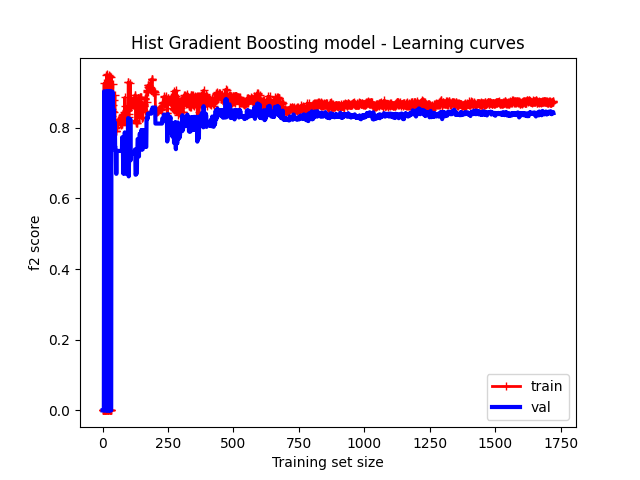
\includegraphics[width=\linewidth]{media/images/learning-curves/hgb.png}
        \caption{Curva de aprendizaje del Hist Gradient Boosting}\ \label{sfig:lc-hgb}
    \end{subfigure}
    \begin{subfigure}[b]{0.3\textwidth}
        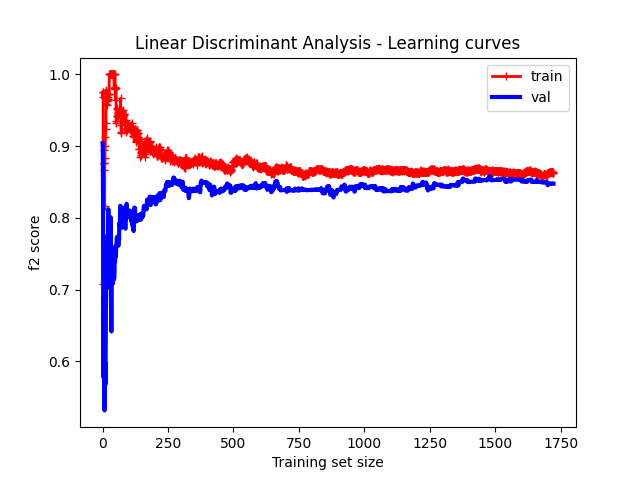
\includegraphics[width=\linewidth]{media/images/learning-curves/lda.png}
        \caption{Curva de aprendizaje del Linear Discriminant Analysis}\ \label{sfig:lc-lda}
    \end{subfigure}
    \begin{subfigure}[b]{0.3\textwidth}
        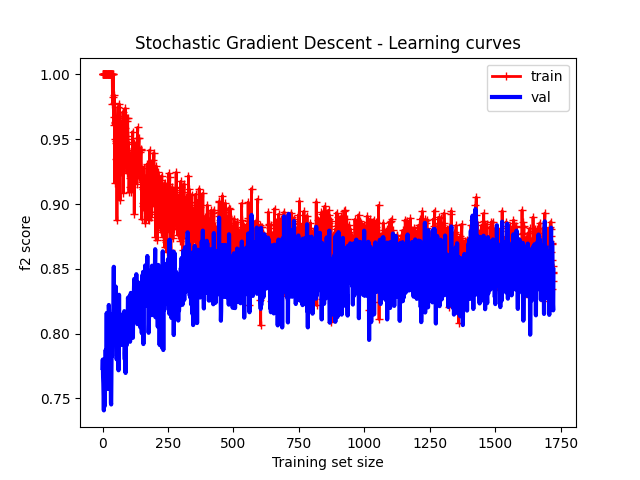
\includegraphics[width=\linewidth]{media/images/learning-curves/sgd.png}
        \caption{Curva de aprendizaje del Stochastic Gradient Descent}\ \label{sfig:lc-sgd}
    \end{subfigure}
    \begin{subfigure}[b]{0.3\textwidth}
        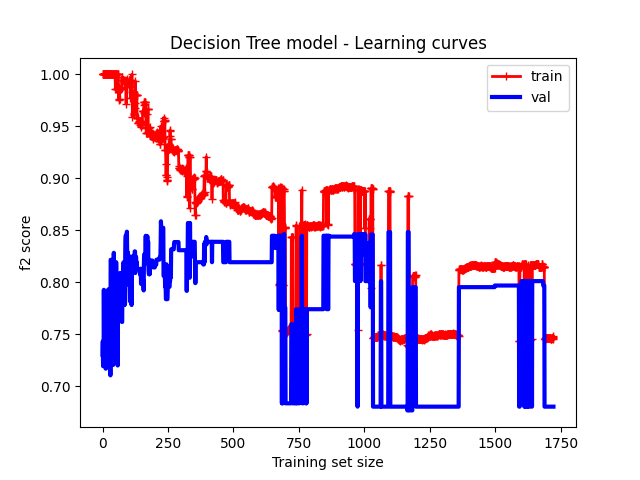
\includegraphics[width=\linewidth]{media/images/learning-curves/dt.png}
        \caption{Curva de aprendizaje del Decision Tree}\ \label{sfig:lc-dt}
    \end{subfigure}
    \caption{Curvas de aprendizaje de los modelos entrenados según el tamaño del \gls{dataset} de entrenamiento. Fuente propia, \textit{código\ \ref{code:plot-learning-curves}}}\ \label{fig:learning-curves}
\end{figure}


\subsubsection{Selección de modelos e \textit{hyperparameter tuning}}\ \label{sec:i1-seleccion}

Antes de elegir el mejor modelo, explicaremos las métricas con los que los evaluamos. Para ello, 

Antes de ajustar los modelos, seleccionaremos aquellos con los mejores resultados. Viendo la \textit{tabla\ \ref{tab:first-model-training}} vemos que los cinco mejores modelos han sido los siguientes:
\begin{enumerate}
    \item Multi-Layer Perceptron
    \item XGBoost
    \item Random Forest
    \item LightGBM
    \item Quadratic Discriminant Analysis
\end{enumerate}

Antes de continuar, descartaremos el \textit{Random Forest}, pues es de los que más tarda en entrenar junto con el \textit{Multi-Layer Perceptron}, sin embargo, a diferencia del segundo, obtenemos peores resultados, aunque se podría trabajar con él de todas formas.

De los cuatro modelos con los que nos hemos quedado al final, solamente dos hacen \gls{overfitting}, de todas formas intentaremos mejorar los resultados de los cuatro. Para ello, primero haremos \href{://scikit-learn.org/stable/modules/generated/sklearn.model_selection.RandomizedSearchCV.html}{RandomizedSearchCV}. Una vez hemos encontrado buenos resultados en el rango de parámetros definido, utilizamos \href{https://scikit-learn.org/stable/modules/generated/sklearn.model_selection.GridSearchCV.html}{GridSearchCV}